\documentclass[12pt]{article}
\usepackage{amsmath,amssymb,amsthm}
\usepackage{fullpage}
\usepackage{graphicx}
\usepackage{hyperref}
\usepackage{url}
\usepackage{booktabs}

\theoremstyle{definition}
\newtheorem{thm}{Theorem}[section]
\newtheorem{lem}[thm]{Lemma}
\newtheorem{corr}[thm]{Corrolary}
\newtheorem{defn}{Definition}[section]
\newtheorem{conj}{Conjecture}[section]
\newtheorem{prob}{Open problem}[section]
\newcommand{\floor}[1]{\left\lfloor #1 \right\rfloor}
\newcommand{\ceil}[1]{\left\lceil #1 \right\rceil}
\newcommand{\bigC}[0]{\mathcal{C}}
\begin{document}
\emergencystretch 3em
\title{A lower bound from a random walk?}

\author{Josh Burdick ({\tt josh.t.burdick@gmail.com})}

\maketitle

\begin{abstract}

Shannon's counting argument \cite{shannon_synthesis_1949} shows that many functions are hard to compute.
However, it is nonconstructive, and so doesn't explicitly state a
hard-to-compute function. Attempts have been made to apply counting arguments to other problems
such as CLIQUE \cite{buggyclique}, without success.
Here, we define a random walk on a $d$-regular graph whose vertices are
sets of cliques. We state a (huge) integer programming
problem which appears to bound the circuit complexity of CLIQUE. We show solutions
of that problem (for {\em tiny} cases -- $n=7, k=3$).

\end{abstract}

\newpage

\tableofcontents

\vspace{5mm}


\section{A random walk on hypergraphs} \label{se:countingBound}

Previously, we considered the set of functions BUGGYCLIQUE, which
only detect a subset of the possible cliques \cite{buggyclique}.
Using a slight modification of Shannon's
function-counting argument \cite{shannon_synthesis_1949},
we showed that a function randomly chosen from BUGGYCLIQUE,
on average, requires $\Omega(n^{k/2})$ two-input NAND gates to compute.

However, that argument didn't give any bound on the complexity of CLIQUE.
It seems that connecting the number of cliques detected by a BUGGYCLIQUE
function, and the number of gates it uses, might be useful. We attempt
to do this using a random walk.

\subsection{Definition of the walk}

Previously, we defined the zeroing-out lattice $Z$, in which all paths lead
``down'' to $\emptyset$. Here, we consider a ``bouncing'' walk
through $Z$, starting from an arbitrary set of cliques $A_t$.

\begin{enumerate}

\item Pick an edge $e$ randomly, and remove all cliques which include it from $A_t$. 
This corresponds to
following a random arc of $Z$ ``down''. Call the resulting set $B_t$ (for ``bounce'').

\item Add a random set of the possible cliques which include $e$,
resulting in a larger set $A_{t+1}$. This corresponds to following
a random arc of $Z$ ``up''.

\item Repeat...

\end{enumerate}

One step of this is depicted in Figure \ref{fig:boing}.

\begin{figure}

\centering

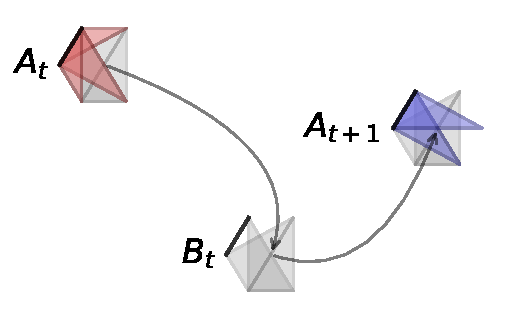
\includegraphics[width=0.5\textwidth]{bounce.pdf}

\caption{
One step of the walk. Starting from $A_t$, the cliques containing 
a randomly-chosen edge are removed, resulting in $B_t$.
Adding a random set of cliques back results in $A_{t+1}$.
}
\label{fig:boing}

\end{figure}

\subsection{Graph-theoretic properties of the walk}
Note that ``one-step reachability'' in the bouncing walk is symmetric;
one step can be an arbitrary modification of which cliques containing 
an edge $e$ are included.
Thus, we can construct a new undirected graph, $S$, with an edge between every
pair of sets of cliques reachable in one step.

\begin{defn} \label{def:bouncingWalk}

Let $Z$ be the previously-defined zeroing-out graph. We will write $Z'$ for
the inverse of that graph (with arrows reversed).

The bouncing walk $S$ is result of following one edge of $Z$, followed by one
edge of $Z'$. Formally, as a relation:

\[
S(a,c) \triangleq \exists b. Z(a,b) \land Z'(b,c)
\]

\end{defn}

We can also characterize $S$ by XORing sets of cliques together.

\begin{defn} \label{def:oneEdgeNeighbors}

Let $A$ be a set of cliques, and let $e$ be an input edge. We write
$e \subset A$ if some clique in $A$ contains the edge $e$.

We define the set of one-edge neighbors $E$, as follows:

\[
E = \emptyset \cup \bigcup_e \{ X: e \subset X\}
\]

\end{defn}

For any given set of cliques $A$, we can generate all the neighbors
of $A$ by picking a set of cliques $X \in E$, and taking $A \oplus X$. This will
add and remove some cliques from $A$, all of which include some edge $e$.
Distinct choices of $X$ will yield distinct neighbors of $A$.
We can enumerate elements of $E$ by picking an edge $e$, 
and then picking any subset of cliques which contains $e$. (This overcounts
elements in $E$, but not by that much; most random sets of cliques won't be
covered by a single edge $e$.) Thus, we have the following bounds for $|E|$:

\[
2^{{n-2} \choose {k-2}} \le |E| \le {n \choose 2} 2^{{n-2} \choose {k-2}}
\]

XORing with something from $E$ defines all of the neighbors of any set of cliques.
Thus, we get that $S$ is a $d$-regular graph, with $d = |E|-1$.
I'm not sure if it's a known $d$-regular graph.
It seems too
dense to be an expander, but does seem to be pretty strongly connected.
$d$-regular graphs have some convenient properties (see e.g. \cite{nilli1991second}).

\subsection{Modelling where the walk goes}

We have two steps, in which cliques are first removed, then added.
As before, let $N = {n \choose k}$.
We also define the number of cliques which potentially could be ``hit'' by
zeroing out an edge as $H = {{n-2} \choose {k-2}}$.

In the first step, when edge $e$ is zeroed out, the number of cliques removed has
a hypergeometric distribution. (This is because $|A_t|$ of the $N$ possible cliques
are present, and we're ``hitting'' $h$ of those when we zero out $e$.)
Thus, for a given $|A_t|$:

\[
P(|A_t - B_t|=d|\hspace{1mm}|A_t|) = \text{Hypergeometric}(d; N, |A_t|, H)
\]

Symmetrically, when we ``bounce'' up, the number of cliques added has
a hypergeometric distribution.

\[
P(|A_{t+1} - B_t|=d|\hspace{1mm}|A_{t+1}|) = \text{Hypergeometric}(d; N, |A_{t+1}|, H)
\]

However, in the second step, before the bounce up, we know that {\em no} cliques contain $e$. The number of
cliques we might add (each chosen uniformly with probability 0.5) has 
a binomial distribution. Thus, we also have that

\[
P(|A_{t+1} - B_t|=d|\hspace{1mm}|B_t|) = \text{Binomial}(d; H, 0.5)
\]

\subsubsection{Number of cliques}

Let $A$ be the $2^N{\times}2^N$ adjacency matrix corresponding to the one-step graph $S$.
We know that $A$ is $d$-regular.
It seems convenient to group together rows and columns of $A$,
which correspond to sets of cliques of the same size.

\begin{defn} \label{defn:levels}

Let $L$ be a $2^N{\times}N$ matrix with rows $i$ corresponding to sets of cliques (indexed arbitrarily), such that
$L_{ij} = 1$ iff the $i$th set contains $j$ cliques. (Here, we assume that column indices are 0-based.)

\end{defn}

Let $L^{\dagger}$ be the Moore-Penrose pseudoinverse of $L$.
We can then define the transition matrix for the walk, with sets of cliques of the same size grouped together.

\begin{defn} \label{defn:B}

Define
$B = L^{\dagger}AL$. This gives the one-step transition probabilities for the walk: $B_{ij}$ is the
probability of going from a set of $i$ cliques to a set of $j$ cliques.

\end{defn}

This summarizes how the walk changes the number of cliques.
Although $B$ is not a $d$-regular graph, it is related to $A$, which is $d$-regular.

\subsubsection{Number of gates}

What can we say about how each step changes the number of gates? Here, the situation is murkier.

First, we define notation for circuit size. 
We only consider using unbounded fan-in NAND gates. (Although
2-input gates are arguably more commonly used in circuit complexity,
unbounded fan-in circuits have been used
\cite{wegener1991complexity}\cite{allender1994depth}.)

\begin{defn} \label{defn:circuitSize}

Define $C_A$ to be the smallest circuit (by number of unbounded fan-in NAND gates)
which detects the set of cliques $A$. ($|C_A|$ is the number of gates in that circuit.)

\end{defn}

\subsubsection{An example}

We first consider what bounds we have for the number of gates,
on one example of a ``bouncing step'' (Figure \ref{fig:boing}).
Here, three cliques were removed in the ``down'' step. Feeding in a 0
to $e$ can't have removed more than three gates, since that many gates would suffice
to convert a circuit detecting $B_t$ into a circuit detecting $A_t$.
So we have a lower bound:

\[
|C_{A_{t+1}}| \ge |C_{B_t}| \ge |C_{A_t}| - 3
\]

And, since two cliques were added in the ``up'' step (requiring no more than two
additional gates to detect), we have an upper bound:

\[
|C_{A_{t+1}}| \le |C_{B_t}| + 2 \le |C_{A_t}| + 2
\]

(Note that using NAND gates, we know that if at least one clique is ``hit'', then
at least one fewer NAND gate is needed. However, this doesn't seem to help much,
and so for simplicity, we ignore this.)

\subsubsection{Bounds for all sets of cliques}

We now attempt to apply that bounding strategy, across all the sets of cliques.
As before, we group the sets of cliques by size.

Let $x_i$ be the expected number of gates needed to detect a set
of $i$ cliques, chosen uniformly at random. (We use 0-based indexing
for $x$.) We will need to consider the number of cliques which are ``hit''
by a random edge.

\begin{defn} \label{defn:sequenceVector}

Define the vector $h = \frac{H}{N}(0, 1, 2, ... N)$. (Again, we use 0-based indexing.)

$h_i$ is the expected number of cliques which would be ``hit'' by zeroing out a random edge
from a set of $i$ cliques (based on its hypergeometric distribution).
Symmetrically, $h_i$ is the expected number of cliques which {\em were just added}, to obtain a
set of $i$ cliques.

\end{defn}

First, we obtain a lower bound on the number of gates after one step.
On the ``down'' step, the expected number of gates ``hit'' is no more than $h$,
and so the expected number of gates remaining is at least $x - h$.
We can't say anything about the number of gates needed to detect additional cliques (in the bounce ``up''), and so we have:
the number of gates after a ``bounce'' is at least $B(x-h)$.

To obtain an upper bound: On the ``down'' step, some number of gates is hit (we don't know how many).
After the bounce, the number of gates is $Bx$.
On the ``up'' step,
if we end up with $i$ cliques, then we know that the expected number of gates added is no more than $h_i$,
and so, in total, we need no more than $Bx+h$ gates.

Thus, we have the following bound (where $\le$ applies element-wise across the vectors):

\begin{equation}
\label{eq:stepBound}
B(x - h) \le x \le Bx + h
\end{equation}

Note that we have an {\em upper} bound on $x$, as well
as a lower bound. Upper bounds have been useful in proving lower bounds;
this recurring theme has been dubbed ``ironic complexity''
\cite{aaronson_pnp}.

These seem to bound $x$ to be somewhat near an eigenvector of $B$. This isn't a very sharp bound.
However, note that for fixed $k$, as $n$ increases, it gets sharper (as $N = {n \choose k}$ increases faster than $H = {{n-2} \choose {k-2}}$).

\subsection{Plotting the walk}

We can plot the effect of one step of this walk, in terms of number of cliques, and number of gates (Figure \ref{fig:walk}).
Note that there is much more uncertainty in the number of gates than the number of cliques. Also, the
uncertainty is higher
for larger sets of cliques.  However, this does suggest that the
number of gates needed is {\em somewhat} related to the number of cliques detected.

\begin{figure}

\centering

\includegraphics[width=1\textwidth]{walking_bounds_0.pdf}

\caption{
Example steps in the bouncing walk, for $n=14, k=4$; 
note that the number of possible cliques $N = {14 \choose 4} = 1,001$.
 Starting from an initial set of cliques ($A_t$, black dot),
a random edge $e$ is chosen. (Note that $e$ could, in general,
``hit'' anywhere from 0 to $H = {12 \choose 2} = 66$ cliques.)
 All cliques containing $e$ are removed, yielding $B_t$ (red region).
Then, a random set of cliques containing $e$ is added back, resulting in $A_{t+1}$ (blue region).
The shading of the regions represents the relative likelihood of different possibilities;
lines indicate bounds on where the walk could go.
The height of the regions reflects the uncertainty in the number
of gates, after a bounce; note that the $y$-axis is relative to the initial number of gates.
}
\label{fig:walk}

\end{figure}


\section{A bound using integer programming?}

We now attempt to obtain a bound on CLIQUE from this random walk, by
writing what we know as a mixed integer program (IP), and then bounding it
using the LP relaxation. Previously, we used an LP \cite{buggyclique}.
(Alternatively, we could solve the IP; however, that seems likely to
be computationally difficult and/or complicated.)

\subsection{Variables and objective function}

First, for a given $n$ and $k$, let $N = {n \choose k}$; this is
the maximum possible number of cliques.

We choose a maximum number of gates $G$ to consider. (If $G$ is
chosen too small, then the problem will be infeasible.)

Then, for $0 \le c \le N$ and $0 \le g \le G$,
we define an integer variable $w_{c,g}$ be the number of functions which contain
exactly $c$ of the possible $N$ cliques, and which require at least
$g$ gates to detect. ($w$ might be considered short for ``weight?'';
it's essentially histogram counts.)

We also define a real-valued variable
$x_c$ as ``expected number of gates needed, for sets of size $c$'':

\[
x_c = \sum_g g \cdot w_{c,g}
\]

Our question: how many gates are in the smallest circuit
which detects {\em all} the cliques? Thus, the objective function
is

\[
\text{Minimize }x_N\text{, subject to the constraints...}
\]

Next, we state the constraints.

\subsection{Counting functions}

Let $m = {n \choose 2}$ be the number of inputs; that is the number
of input edges for an $n$-vertex graph.

We have the counting argument: the number of $m$-input functions
constructable using $g$ gates is bounded. (This number increases
quickly as a function of $g$, but nonetheless is bounded.)
Here, we only consider unbounded fan-in NAND gate circuits. For
this sort of circuit, we have the bound:

\[
\sum_c w_{c,g} \le 2^{\sum_{i=0}^{g-1} m+i}
\]

We might think of the set of functions as filling a conical
martini glass. If we consider the $z$ axis to be ``number of gates'',
then there is ``room for more functions higher up.''

\subsection{Counting sets of cliques}

We also know the number of sets of cliques (and thus, the number
of BUGGYCLIQUE functions) for a given number of cliques $c$.

\[
\sum_g w_{c,g} = {N \choose c}
\]

Note that this has a sharp maximal peak at $c = N/2$.

\subsection{The walking bound}

We can also add the walking bound (equation \ref{eq:stepBound}), which bounds how much
one ``step'' of the walk can affect the number of gates.
We compute the matrix $B$, the vector $h$, and then add a constraint for each element of $x_i$.

\subsection{Bound on finding zero cliques}

We also have a slightly comical upper bound:
to detect zero cliques, we simply always
output a 0. We can implement this with one NAND gate (or possibly zero;
I'm not quite sure how to count this). We refer to this as the
``no cliques'' constraint. We have:

\[
x_0 = 1
\]

Why might we think that this is even {\em remotely} useful? We are, after
all, trying to bound $x_N$...

Well, we know that if we start at $c=0$ cliques, if a random walk takes us to
$c \approx N/2$ cliques, then at that point, the counting bound implies that
(on average), we'll need a large-ish number of gates to detect those $c$ cliques.
The walking bound limits how much the number of gates can fluctuate
in getting there. Thus, forcing $x_0=1$ should ``drag down'' the left-hand side of the graph.

My intuition is that functions with smaller numbers for $c$ would
tend to ``fill up'' the space available for functions with smaller numbers of gates.
(Recall that when we use fewer gates, we reduce the number of functions we can implement.)
Hopefully this would ``rule out'' things in the right-hand side of the graph (such as CLIQUE)
from having a small number of gates.

\section{Results}

We solved the LP relaxation of the IP problem (using GLPK \cite{glpk})
for a {\em tiny} instance, $n=7, k=3$, and allowing up to 3 (unbounded fan-in)
NAND gates.
Figure \ref{fig:bounds0} shows results thus far.
Note that unlike previous related bounds, here we {\em only} solve minimizing
$x_N$, and plot the resulting bounds $x_j$, at that solution. The
goal here is to see what the LP considers a possible scenario, when
minimizing the number of gates for CLIQUE.

\begin{figure}

\centering

\includegraphics[width=0.9\textwidth]{bounds\_7\_3\_3.pdf}

\caption{
Bounds with $n=7$ and $k=3$, including different sets of constraints.
Note that this plot shows results for all the variables, when
minimizing $x_N$.
}
\label{fig:bounds0}

\end{figure}

In general, there could be many possible solutions to the LP, which
limits how much we can draw conclusions from this plot.
However, parts of this plot make sense: 
when the ``step'' and ``no cliques''
constraints are added (green line), the largest number of gates is shifted
slightly to the right (towards a larger number of cliques).

On larger instances, the LP crashes (using several different solvers). This
is presumably partly because the numbers in the IP add up to $2^{n \choose k}$,
which grows very quickly.

This raises the following open question:

\begin{prob}
What bound would this give for CLIQUE, if the LP {\em didn't} crash?
\end{prob}

\section{Conclusion}

We attempt to bound the circuit complexity of CLIQUE using an integer program.
Currently, this gives a bound
of 1 unbounded fan-in NAND gate for CLIQUE...

Solving the integer program directly seems impractical, as it has well over
${n \choose k}$ variables. This raises the question of whether we can prove
anything about the IP, without explicitly solving it.
The walk which we defined is on a $d$-regular graph, and we have some bounds on
how much the number of cliques (and number of gates needed to detect them)
changes on each step. However, we haven't been able to use these properties
to obtain a lower bound.

\section{Acknowledgements}

The emphasis on random walks was partly inspired by the late Luca
Trevisan's blog, {\em in theory}; as many complexity commentators
have noted, he will be missed. The author would also like to thank
the authors and maintainers of several other entertaining and
relevant blogs, including but not limited to: the Computational
Complexity blog (Lance Fortnow and William Gasarch), Emanuele Viola's
blog Thoughts, G\"odel's Lost Letter (Richard Lipton and Ken Regan),
and Shtetl-Optimized (Scott Aaronson),

\bibliography{references}
\bibliographystyle{unsrt}

\end{document}

